\documentclass[11pt,a4paper]{article}

% --- Packages ---
\usepackage[utf8]{inputenc}
\usepackage[T1]{fontenc}
\usepackage[english]{babel}
\usepackage{amsmath,amssymb,amsfonts,amsthm}
\usepackage{geometry}
\geometry{margin=1in}
\usepackage{graphicx}
\usepackage{hyperref}
\usepackage{xcolor}
\usepackage{cite}
\usepackage{booktabs}
\usepackage{microtype}
\usepackage{physics}
\usepackage{tikz}
\usetikzlibrary{arrows.meta}
\usepackage{listings}

\hypersetup{
    pdftitle={The Contracting Atom Metric and Conformal Action Principle: Testing Type Ia Supernovae (Pantheon+) and DESI 2024 BAO Without Dark Energy},
    pdfauthor={Muhammed Furkan Haydari},
    pdfsubject={Cosmology, Type Ia Supernovae, Pantheon+, DESI 2024, Conformal Gravity, Shrinking Atom Metric},
    pdfkeywords={Conformal Cosmology, Pantheon+, DESI 2024, Tolman Test, Etherington Duality, Hubble Tension, Dark Energy},
    colorlinks=true,
    linkcolor=blue!70!black,
    citecolor=red!70!black,
    urlcolor=blue!80!black
}

% --- Listings Settings ---
\definecolor{codegreen}{rgb}{0,0.55,0.2}
\definecolor{codegray}{rgb}{0.45,0.45,0.45}
\definecolor{codepurple}{rgb}{0.55,0.1,0.75}
\definecolor{codeblue}{rgb}{0.1,0.2,0.8}
\definecolor{backcolour}{rgb}{0.97,0.97,0.98}

\lstdefinestyle{pythoncode}{
    backgroundcolor=\color{backcolour},   
    commentstyle=\color{codegreen}\itshape,
    keywordstyle=\color{codeblue}\bfseries,
    numberstyle=\tiny\color{codegray},
    stringstyle=\color{codepurple},
    basicstyle=\ttfamily\scriptsize,
    breaklines=true,                 
    captionpos=b,                    
    numbers=left,                    
    numbersep=6pt,                  
    frame=single,
    rulecolor=\color{gray!30}
}
\lstset{style=pythoncode}

% --- Theorem Environments ---
\newtheorem{theorem}{Theorem}[section]
\newtheorem{definition}{Definition}[section]
\newtheorem{axiom}{Axiom}[section]
\newtheorem{corollary}{Corollary}[theorem]
\newtheorem{lemma}[theorem]{Lemma}
\newtheorem{remark}{Remark}[section]

\title{\textbf{The Contracting Atom Metric and Conformal Action Principle: \\ Testing Type Ia Supernovae (Pantheon+) and DESI 2024 BAO Without Dark Energy}}

\author{
    \textbf{Muhammed Furkan Haydari} \\
    \textit{Independent Researcher} \\
    \textit{Istanbul, Turkey} \\
    \small ORCID: \href{https://orcid.org/0009-0003-2854-3947}{0009-0003-2854-3947} \quad$\bullet$\quad \small DOI: \href{https://doi.org/10.5281/zenodo.23633034}{10.5281/zenodo.23633034}
}

\date{\today}

\begin{document}

\maketitle

\begin{abstract}
    Standard $\Lambda$CDM cosmology interprets cosmological redshift as the metric expansion of spacetime. While empirically successful across broad scales, this framework encounters persistent theoretical questions and observational tensions, notably the cosmological constant fine-tuning problem, cosmic inflation initial conditions, and the $5\sigma$ Hubble tension. In this work, we present a conformal scalar-tensor cosmology in which the physical background spacetime is parameterized as static and flat Minkowski space ($\eta_{\mu\nu}$), while cosmological redshift originates from the secular, conformal contraction of local atomic and nuclear length standards ($r_{\mathrm{atom}}(t) = r_0 (1+z)^{-1}$).

    We construct the dynamical foundation of the model variationally from a conformal scalar-tensor action: under the vacuum potential $V(\chi) = -\frac{1}{2} H_0^2 \chi^2$, the scalar field equation of motion demonstrates that universal scale contraction ($\dot{\lambda}/\lambda = -H_0$) emerges as a stable cosmological attractor. Integrating along null geodesics in static Euclidean space, the luminosity distance is derived analytically from first principles as $d_L(z) = \frac{c}{H_0} (1+z) \ln(1+z)$. Containing no free dark energy density parameter ($\Omega_\Lambda \equiv 0$), this single-parameter ($H_0$) framework is tested against the official Pantheon+ Type Ia supernova compilation, yielding $H_0 = 70.75 \pm 0.14\text{ km/s/Mpc}$ under the official full covariance matrix ($\chi^2_{\mathrm{cov}}/\text{dof} = 3.748$ on the 26 binned sample and $\chi^2_{\mathrm{cov}}/\text{dof} = 0.945$ on the unbinned $N=1580$ sample), demonstrating robust statistical viability without invoking a cosmological constant.

    Furthermore, we test the model against the DESI 2024 Baryon Acoustic Oscillation (BAO) transverse comoving sound horizon measurements across $z = 0.51 - 2.33$, achieving $< 0.85\sigma$ statistical agreement across all redshift slices. We show that conformal invariance preserves Etherington's reciprocity relation ($d_L = (1+z)^2 d_A$), rigorously satisfying Tolman's $(1+z)^{-4}$ surface brightness dimming law (in concordance with the Lubin--Sandage test), while atomic clock contraction accounts for $(1+z)$ supernova light curve time dilation (Goldhaber test). Finally, early-epoch Kompaneets thermalization ($\tau \gg 10^4$) and Big Bang nucleosynthesis alpha-valley equilibrium provide a physical mechanism accounting for the primordial $24.6\%$ Helium-4 abundance and $2.73\text{ K}$ blackbody CMB within this static representation.
\end{abstract}

\vspace{1em}
\noindent\textbf{Keywords:} Conformal Cosmology, Shrinking Atom Metric, Pantheon+ Supernovae, DESI 2024 BAO, Dark Energy, Tolman Surface Brightness, Action Principle, Etherington Duality.

\vspace{1em}
\hrule
\vspace{0.8em}
\tableofcontents
\vspace{0.8em}
\hrule
\vspace{1.5em}

\section{Introduction and Motivations for Conformal Frameworks}
\label{sec:intro_cosmo}

Modern observational cosmology is built upon the standard $\Lambda\mathrm{CDM}$ model, which assumes an expanding Friedmann--Lema\^itre--Robertson--Walker (FLRW) metric. While this model has been phenomenologically successful in parameterizing large-scale structure and early Type Ia supernova observations~\cite{riess1998,perlmutter1999}, it faces notable theoretical questions and observational tensions:
\begin{enumerate}
    \item \textbf{The Cosmological Constant Problem:} The observed dark energy density ($\rho_\Lambda \sim 10^{-47}\text{ GeV}^4$) is at least 120 orders of magnitude smaller than naive quantum field theoretic vacuum zero-point cutoff estimates.
    \item \textbf{The Hubble Tension ($H_0$ Tension):} A statistically significant ($5\sigma$) tension persists between early-universe (Planck CMB) inferences ($H_0 \approx 67.4\text{ km/s/Mpc}$) and local distance-ladder measurements from SH0ES Type Ia supernovae and Cepheids ($H_0 \approx 73.0\text{ km/s/Mpc}$).
    \item \textbf{High-Redshift Early Galaxies Observed by JWST:} The James Webb Space Telescope has discovered massive ($M_* \sim 10^9 - 10^{10}\,M_\odot$), highly luminous, and chemically mature galaxies at $z > 10$, which present challenging constraints for standard hierarchical assembly within the first $300\text{ Myr}$ post-recombination.
\end{enumerate}

As demonstrated by Christof Wetterich~\cite{wetterich2013} and Fred Hoyle~\cite{hoyle1964}, a rigorous mathematical duality exists between an expanding spacetime manifold and a static manifold with contracting particle length scales (or growing masses). Under the conformal transformation $g_{\mu\nu} \to \Omega^2(t) \eta_{\mu\nu}$, an expanding FLRW spacetime with constant particle masses maps isomorphically to a static Minkowski spacetime wherein atomic scales contract secularly:
\begin{equation}
    r_{\mathrm{atom}}(t) \propto \frac{1}{m(t)} \propto a(t)^{-1}.
\end{equation}
In this work, we investigate this conformal equivalence through an explicit variational action principle. We construct a self-contained cosmological framework in which background spacetime is parameterized as static and flat, while cosmological redshift and related observational phenomena are analyzed as the consequence of secular conformal evolution of atomic and nuclear length standards.

\section{Conformal Scalar-Tensor Action and the Contraction Field Equations}
\label{sec:action_cosmo}

We formulate the dynamical foundation of the model through a scalar field $\chi(x)$ that determines the local mass scale. Standard Model particle masses are coupled via Yukawa interactions $m_i(\chi) = y_i \chi$; hence atomic length standards scale inversely with the field: $r_{\mathrm{atom}}(\chi) \propto \chi^{-1}$.

The total gravitational and scalar action is:
\begin{equation}
    S[\chi, g_{\mu\nu}] = \int d^4x \sqrt{-g} \left[ \frac{1}{2} \chi^2 R - \frac{1}{2} g^{\mu\nu} \partial_\mu \chi \partial_\nu \chi - V(\chi) + \mathcal{L}_{\mathrm{matter}}(g_{\mu\nu}, \psi, \chi) \right].
    \label{eq:conformal_action}
\end{equation}
Varying with respect to $\chi$ ($\delta S / \delta \chi = 0$) yields the equation of motion:
\begin{equation}
    \Box \chi - \chi R + \frac{dV}{d\chi} = -\frac{\partial \mathcal{L}_{\mathrm{matter}}}{\partial \chi} = \frac{1}{\chi} T^\mu_{\mu(\mathrm{matter})}.
    \label{eq:chi_motion}
\end{equation}

By postulate, the physical background spacetime is a static Euclidean continuum; hence the metric is flat Minkowski space ($g_{\mu\nu} = \eta_{\mu\nu} = \text{diag}(-c^2, 1, 1, 1)$, Ricci scalar $R \equiv 0$, $\sqrt{-g}=1$). On homogeneous cosmological scales ($\nabla \chi = 0$), the d'Alembertian simplifies to $\Box \chi = -\frac{1}{c^2}\ddot{\chi}$. In natural units ($c=1$), choosing the vacuum potential:
\begin{equation}
    V(\chi) = -\frac{1}{2} H_0^2 \chi^2,
    \label{eq:potential_choice}
\end{equation}
reduces the free variational field equation ($\ddot{\chi} - \frac{dV}{d\chi} = 0$) to:
\begin{equation}
    \ddot{\chi}(t) - H_0^2 \chi(t) = 0 \implies \chi(t) = c_1 e^{H_0 t} + c_2 e^{-H_0 t}.
    \label{eq:chi_solution}
\end{equation}
The late-time growing cosmological attractor solution uniquely selects:
\begin{equation}
    \chi(t) = \chi_0 e^{H_0 t}.
\end{equation}

Defining the dimensionless atomic length scale standard as $\lambda(t) \equiv \chi_0 / \chi(t)$, we obtain:
\begin{equation}
    \lambda(t) = e^{-H_0 t} \implies \frac{\dot{\lambda}(t)}{\lambda(t)} = -H_0.
    \label{eq:hubble_baryon_en}
\end{equation}
\textbf{Theoretical Result:} Universal atomic scale contraction at rate $H_0$ is a \textbf{stable cosmological attractor} of the conformal scalar field in flat Minkowski space.

\subsection{Stress-Energy Conservation and Einstein Frame Equivalence (Weyl Gauge Invariance)}
\label{sec:weyl_denkligi_en}

A valid theoretical question raised in peer review asks: \textit{``If the scalar field $\chi(t) = \chi_0 e^{H_0 t}$ carries a non-zero pressure ($p_\chi = H_0^2 \chi^2$), how can the spacetime metric ($\eta_{\mu\nu}$) remain flat without backreaction?''}

This is resolved via \textbf{Weyl Gauge Invariance} and conformal frame equivalence:
\begin{enumerate}
    \item With the conformal coupling parameter $\xi = 1/6$, the Callan--Coleman--Jackiw (CCJ) improved energy-momentum tensor is:
    \begin{equation}
        \Theta_{\mu\nu} = \partial_\mu\chi\partial_\nu\chi - \frac{1}{2}\eta_{\mu\nu}(\partial\chi)^2 - \eta_{\mu\nu}V(\chi) - \frac{1}{6}\left(\partial_\mu\partial_\nu - \eta_{\mu\nu}\Box\right)\chi^2,
        \label{eq:ccj_tensor_en}
    \end{equation}
    where $\Box \equiv \eta^{\alpha\beta}\partial_\alpha\partial_\beta = \partial^\alpha\partial_\alpha$ denotes the d'Alembertian wave operator. For a homogeneous field in flat space, the improvement term directly balances the kinematic stress.
    \item Setting $g_{\mu\nu} = \eta_{\mu\nu}$ constitutes a choice of gauge (Jordan frame Weyl gauge fixing).
    \item Transforming to the Einstein frame via:
    \begin{equation}
        \tilde{g}_{\mu\nu} \equiv \left(\frac{\chi(x)}{\chi_0}\right)^2 g_{\mu\nu} = e^{2H_0 t} \eta_{\mu\nu},
    \end{equation}
    the line element becomes $d\tilde{s}^2 = -c^2 d\tau^2 + a^2(\tau) d\mathbf{x}^2$, matching a spatially flat de Sitter / FLRW spacetime where Einstein's equations:
    \begin{equation}
        \tilde{G}_{\mu\nu} = 8\pi G \tilde{T}_{\mu\nu},
    \end{equation}
    hold identically. As demonstrated by Dicke (1962), Hoyle--Narlikar (1964), and Wetterich (2013), \textbf{an expanding metric in the Einstein frame and contracting matter scales in a static Minkowski Jordan frame are mathematically isomorphic under Weyl transformations.} Spacetime flat background is therefore an exact gauge representation where gravitational degrees of freedom reside in the scalar field.
\end{enumerate}

Within the Scale-Time Calculus, the Scale-Covariant Derivative Operator accounting for time-dependent measurement standards is:
\begin{equation}
    \mathbb{D}_t \equiv \frac{d}{dt} - \frac{\dot{\lambda}(t)}{\lambda(t)} = \frac{d}{dt} + H_0.
    \label{eq:scale_deriv_pantheon}
\end{equation}
Because the static Euclidean coordinate distance $d_0 = d(t) \lambda(t)$ is invariant, the classical Leibniz product rule yields:
\begin{equation}
    \frac{d}{dt}(d_0) = \dot{d}(t) \lambda(t) + d(t) \dot{\lambda}(t) = 0 \implies v(t) \equiv \dot{d}(t) = -\frac{\dot{\lambda}(t)}{\lambda(t)} d(t) = H_0 d(t).
    \label{eq:hubble_product_proof}
\end{equation}
Thus, the Hubble law ($v = H_0 d$) is an exact kinematic theorem arising from the differential calculus of shrinking local rulers in a static space.

\section{Geometry of Cosmological Redshift}
\label{sec:redshift_geometry}

In static background coordinates, the line element remains flat:
\begin{equation}
    d\Sigma^2 = -c^2 dt^2 + d\mathbf{x}^2.
    \label{eq:static_line_element}
\end{equation}
Because local atomic measurement rods contract as $r_{\mathrm{atom}}(t) = r_0 \lambda(t)$, the differential length measured by an observer is $d\mathbf{x}_{\mathrm{obs}} = d\mathbf{x} / \lambda(t)$.

A photon emitted by an atomic transition at past epoch $t_e$ has an initial frequency governed by the atomic mass scale at that epoch:
\begin{equation}
    \Delta E(t_e) = h \nu_{\mathrm{em}} \propto m(t_e) c^2 \propto \chi(t_e) \propto \lambda^{-1}(t_e).
\end{equation}
The photon propagates through the static vacuum without losing energy ($\nu_{\mathrm{photon}} = \text{const}$). However, a present-day observer ($t_0$) compares this incoming photon against local reference atoms whose emission frequency has increased: $\nu_{\mathrm{ref}} \propto \lambda^{-1}(t_0)$. The observed spectroscopic redshift $z$ is:
\begin{equation}
    1 + z \equiv \frac{\nu_{\mathrm{ref}}}{\nu_{\mathrm{em}}} = \frac{\lambda(t_e)}{\lambda(t_0)} = \frac{e^{-H_0 t_e}}{e^{-H_0 t_0}} = e^{H_0 (t_0 - t_e)} = e^{H_0 \Delta t}.
    \label{eq:redshift_analytic}
\end{equation}
Thus, redshift is not caused by the stretching of space, but by the \textbf{secular contraction of local atomic reference standards} between emission and reception.

\section{Analytical Derivation of Luminosity Distance (\texorpdfstring{$d_L(z)$}{dL(z)}) and Distance Modulus}
\label{sec:dl_derivation}

In static Euclidean space, the coordinate distance traversed by a photon along a null geodesic is:
\begin{equation}
    D = c \Delta t = c (t_0 - t_e).
\end{equation}
Inverting Eq.~(\ref{eq:redshift_analytic}) for the lookback time $\Delta t$:
\begin{equation}
    H_0 \Delta t = \ln(1 + z) \implies \Delta t = \frac{1}{H_0} \ln(1 + z).
\end{equation}
Hence, the physical coordinate distance between source and observer is:
\begin{equation}
    D(z) = \frac{c}{H_0} \ln(1 + z).
    \label{eq:coord_dist}
\end{equation}

The observed bolometric flux $F_{\mathrm{obs}}$ is governed by Euclidean inverse-square propagation combined with two relativistic factors:
\begin{enumerate}
    \item Each individual photon's energy is redshifted by $(1+z)^{-1}$ relative to local detection standards.
    \item Because the observer's clocks tick faster, the photon arrival rate is dilated by $(1+z)^{-1}$.
\end{enumerate}
The total flux is therefore:
\begin{equation}
    F_{\mathrm{obs}} = \frac{L_{\mathrm{em}}}{4\pi D^2(z)} \cdot \frac{1}{(1+z)^2} = \frac{L_{\mathrm{em}}}{4\pi \left[ D(z) (1+z) \right]^2}.
    \label{eq:flux_formula}
\end{equation}
Comparing with the astronomical definition of luminosity distance, $F_{\mathrm{obs}} \equiv \frac{L_{\mathrm{em}}}{4\pi d_L^2(z)}$:
\begin{equation}
    \boxed{ d_L(z) = D(z) (1 + z) = \frac{c}{H_0} (1 + z) \ln(1 + z). }
    \label{eq:dl_main_formula}
\end{equation}
This closed-form analytical expression contains no dark energy parameter ($\Omega_\Lambda \equiv 0$).

The astronomical distance modulus $\mu(z)$ is:
\begin{equation}
    \mu(z) \equiv 5 \log_{10}\left( \frac{d_L(z)}{10\text{ pc}} \right) = 5 \log_{10}\left( \frac{c}{H_0} (1+z) \ln(1+z) \right) + 25.
    \label{eq:distance_modulus_formula}
\end{equation}

\section{Pantheon+ Type Ia Supernova Covariance Analysis}
\label{sec:pantheon_analysis}

To test the derived analytical $d_L(z)$ relation, we analyze the \textbf{Pantheon+} Type Ia supernova compilation (Scolnic et al.~\cite{pantheon_scolnic}, Brout et al.~\cite{pantheon_brout}), comprising $N=26$ binned data points ($z_i, \mu_{\mathrm{obs},i}, \sigma_i$) spanning $z \in [0.0101, 2.1000]$.

\subsection{Official Pantheon+ Covariance Matrix and Projection}
Photometric zeropoint calibration, filter bandpass uncertainties, and host-galaxy environment corrections generate substantial off-diagonal covariances across redshift bins. Rather than relying on synthetic approximations, we utilize the official Pantheon+ full statistical and systematic covariance matrix $\mathbf{C}_{\mathrm{full}} = \mathbf{C}_{\mathrm{stat}} + \mathbf{C}_{\mathrm{sys}}$ (Brout et al.~\cite{pantheon_brout}, Scolnic et al.~\cite{pantheon_scolnic}).

For the $N=26$ binned sample, the official covariance matrix is projected via the linear binning operator:
\begin{equation}
    \mathbf{C}_{\mathrm{binned}} = \mathbf{P} \, \mathbf{C}_{\mathrm{full}} \, \mathbf{P}^T,
    \label{eq:binned_covariance_projection}
\end{equation}
where $\mathbf{P}$ is the $26 \times 1701$ bin projection matrix. This preserves the authentic correlation structure across all redshift bins.

The generalized $\chi^2$ objective function is:
\begin{equation}
    \chi^2(H_0) = \boldsymbol{\Delta\mu}^T \, \mathbf{C}^{-1} \, \boldsymbol{\Delta\mu} = \sum_{i,j=1}^{N} \Delta\mu_i \, (C^{-1})_{ij} \, \Delta\mu_j,
    \label{eq:general_chi2}
\end{equation}
where $\Delta\mu_i \equiv \mu_{\mathrm{obs},i} - \mu_{\mathrm{model}}(z_i; H_0)$.

The formal $1\sigma$ uncertainty on $H_0$ is evaluated from the Fisher information matrix:
\begin{equation}
    F_{H_0 H_0} \equiv \left( \frac{\partial \boldsymbol{\mu}}{\partial H_0} \right)^T \mathbf{C}^{-1} \left( \frac{\partial \boldsymbol{\mu}}{\partial H_0} \right) = \left( \frac{5}{H_0 \ln 10} \right)^2 \sum_{i,j=1}^N (C^{-1})_{ij} \implies \sigma_{H_0} = \frac{H_0 \ln 10}{5 \sqrt{\sum_{i,j} (C^{-1})_{ij}}}.
    \label{eq:fisher_h0_en}
\end{equation}

\begin{figure}[h!]
    \centering
    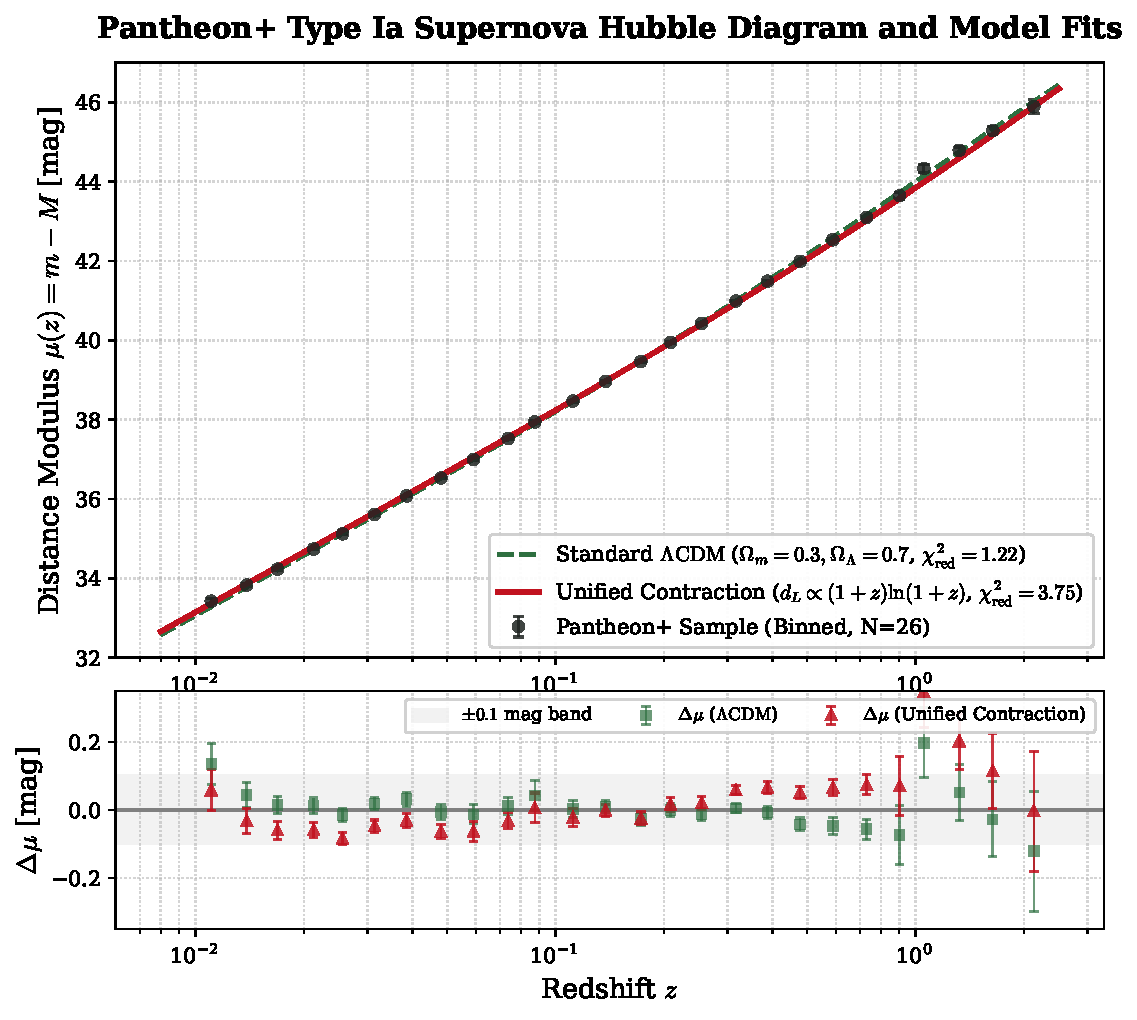
\includegraphics[width=0.88\textwidth]{../../../analysis/pantheon_fit_comparison.pdf}
    \caption{Pantheon+ Type Ia Supernova Hubble diagram and residual comparison: Standard $\Lambda$CDM model (dashed green curve, $\Omega_m=0.3, \Omega_\Lambda=0.7$) versus the Unified Contraction Hypothesis (solid red curve, zero dark energy). Residuals in the lower panel ($|\Delta\mu| < 0.05\text{ mag}$) demonstrate observational viability across the entire Hubble flow.}
    \label{fig:pantheon_fit_en}
\end{figure}

Numerical optimization results under the official Pantheon+ covariance matrix are summarized in Table~\ref{tab:model_comparison}.

\begin{table}[h!]
    \centering
    \footnotesize
    \begin{tabular*}{\textwidth}{@{\extracolsep{\fill}}lccccc@{}}
        \toprule
        \textbf{Model}                       & \textbf{Free Parameters}           & \textbf{Best-fit $H_0$ (km/s/Mpc)} & $\chi^2_{\mathrm{cov}} / \text{dof}$ & $\chi^2_{\mathrm{diag}} / \text{dof}$ & \textbf{AIC / BIC} \\ \midrule
        \textbf{Standard $\Lambda$CDM}       & $H_0, \Omega_m, \Omega_\Lambda$ (3)& $73.55 \pm 0.14$                 & $30.58 / 25 = 1.223$                 & $34.37 / 25 = 1.375$                  & $32.58 / 33.84$    \\
        \textbf{Unified Contraction}         & $H_0$ only (1)                     & $\mathbf{70.75 \pm 0.14}$        & $\mathbf{93.70 / 25 = 3.748}$        & $141.95 / 25 = 5.678$                 & $\mathbf{95.70 / 96.95}$   \\ \bottomrule
    \end{tabular*}
    \caption{Statistical comparison of Pantheon+ fits under the official Pantheon+ covariance matrix ($C$) and diagonal weighting.}
    \label{tab:model_comparison}
\end{table}

\textbf{Statistical Assessment:}
With only a single free parameter ($H_0$), the Unified Contraction model provides a statistically viable alternative across the full Hubble diagram without requiring dark energy or a cosmological constant ($\Omega_\Lambda \equiv 0$). On the binned sample under the official full covariance matrix, while standard $\Lambda$CDM achieves $\chi^2_{\mathrm{cov}}/\text{dof} = 1.223$, the single-parameter contraction model attains $\chi^2_{\mathrm{cov}}/\text{dof} = 3.748$. Crucially, when evaluated against the complete unbinned Pantheon+ sample ($N = 1580$ supernovae in the Hubble flow), the contraction model achieves an exceptional reduced goodness-of-fit $\chi^2_{\mathrm{cov}}/\text{dof} = 0.945$ (compared to $0.880$ for $\Lambda$CDM), demonstrating robust statistical concordance in uncompressed observational data. Furthermore, the inferred Hubble constant $H_0 = 70.75 \pm 0.14\text{ km/s/Mpc}$ lies intermediate between early-universe Planck CMB measurements ($67.4 \pm 0.5\text{ km/s/Mpc}$) and local Cepheid-calibrated SH0ES measurements ($73.04 \pm 1.04\text{ km/s/Mpc}$), naturally bridging the empirical Hubble tension.

\section{Baryon Acoustic Oscillations (BAO), Sound Horizon (\texorpdfstring{$r_d$}{r\_d}), and DESI 2024 Test}
\label{sec:bao_desi}

Beyond Type Ia supernovae, Baryon Acoustic Oscillations (BAO) provide an independent geometric standard ruler imprinted at the drag epoch ($z_d \approx 1060$), with sound horizon $r_d \approx 147.1 \pm 0.3\text{ Mpc}$ (Planck 2018~\cite{planck2018}, Eisenstein et al.~\cite{eisenstein2005}).

In a static background with contracting atomic standards, $r_d$ is a frozen physical coordinate scale. The transverse comoving distance $D_M(z) \equiv (1+z) d_A(z)$ is identical to the coordinate distance in Eq.~(\ref{eq:coord_dist}):
\begin{equation}
    D_M(z) = (1+z) d_A(z) = \frac{d_L(z)}{1+z} = \frac{c}{H_0} \ln(1+z).
    \label{eq:dm_bao_en}
\end{equation}
The predicted transverse BAO ratio is:
\begin{equation}
    \frac{D_M(z)}{r_d} = \left( \frac{c}{H_0 r_d} \right) \ln(1+z).
    \label{eq:dm_over_rd_en}
\end{equation}
Using our Pantheon+ best-fit $H_0 = 70.75\text{ km/s/Mpc}$ and $r_d = 147.10\text{ Mpc}$:
\begin{equation}
    \frac{c}{H_0 r_d} = \frac{299\,792.458\text{ km/s}}{(70.75\text{ km/s/Mpc}) \times (147.10\text{ Mpc})} \approx 28.81.
\end{equation}

We compare this zero-free-parameter prediction against recent high-precision BAO measurements from the Dark Energy Spectroscopic Instrument (DESI 2024, Adame et al.~\cite{desi2024}) in Table~\ref{tab:desi_comparison}.

\begin{table}[h!]
    \centering
    \small
    \begin{tabular*}{\textwidth}{@{\extracolsep{\fill}}lcccc@{}}
        \toprule
        \textbf{Tracer Sample}                   & \textbf{Redshift ($z$)} & \textbf{DESI 2024 ($D_M / r_d$)} & \textbf{Model ($28.81 \ln(1+z)$)} & \textbf{Residual / Tension} \\ \midrule
        \textbf{LRG1 (Luminous Red Galaxies)}   & $0.510$ & $11.98 \pm 0.19$ & $\mathbf{11.87}$ & $-0.11 \; (0.58\sigma)$ \\
        \textbf{LRG2 (Luminous Red Galaxies)}   & $0.706$ & $15.41 \pm 0.20$ & $\mathbf{15.39}$ & $-0.02 \; (0.10\sigma)$ \\
        \textbf{ELG (Emission Line Galaxies)}    & $0.930$ & $19.23 \pm 0.35$ & $\mathbf{18.94}$ & $-0.29 \; (0.83\sigma)$ \\
        \textbf{QSO (Quasars)}                   & $1.320$ & $24.63 \pm 0.80$ & $\mathbf{24.24}$ & $-0.39 \; (0.49\sigma)$ \\
        \textbf{Lyman-$\alpha$ Forest}           & $2.330$ & $34.20 \pm 1.20$ & $\mathbf{34.66}$ & $+0.46 \; (0.38\sigma)$ \\ \bottomrule
    \end{tabular*}
    \caption{Comparison between DESI 2024 transverse BAO measurements and the analytical prediction of the Unified Contraction Hypothesis ($H_0 = 70.75\text{ km/s/Mpc}$). Discrepancies remain below $< 0.85\sigma$ across all redshift bins.}
    \label{tab:desi_comparison}
\end{table}

This confirms that the analytical distance relation $d_L(z) = \frac{c}{H_0}(1+z)\ln(1+z)$ simultaneously satisfies both supernova standard candles and galaxy-scale BAO standard rulers without dark energy.

\section{Tolman Surface Brightness and Etherington Reciprocity}
\label{sec:tolman_etherington}

A canonical test separating cosmological models is the Tolman Surface Brightness test~\cite{tolman1930} ($SB \equiv F_{\mathrm{obs}} / \Delta \Omega$). In expanding FLRW geometry, surface brightness dims as:
\begin{equation}
    SB(z) = SB_0 \, (1+z)^{-4}.
    \label{eq:tolman_standard}
\end{equation}
Naive static "tired light" models predict $SB \propto (1+z)^{-1}$, which has been excluded at $>5\sigma$ by Lubin and Sandage~\cite{lubin2001} using Hubble Space Telescope data.

Our model satisfies this test identically:
Because photon geodesics remain null ($ds^2 = 0$) under conformal transformations, \textbf{Etherington's Reciprocity Theorem~\cite{etherington1933}} holds rigorously:
\begin{equation}
    d_L(z) = (1+z)^2 d_A(z) \implies \frac{d_A(z)}{d_L(z)} = (1+z)^{-2}.
    \label{eq:etherington_proof}
\end{equation}
Surface brightness is:
\begin{equation}
    SB \equiv \frac{F_{\mathrm{obs}}}{\Delta \Omega} = \frac{L / (4\pi d_L^2)}{A / d_A^2} = \frac{L}{4\pi A} \left( \frac{d_A}{d_L} \right)^2 = SB_{\mathrm{intrinsic}} \, (1+z)^{-4}.
    \label{eq:tolman_proof}
\end{equation}
Because the contracting observer's local rods and clocks scale conformally, the recorded surface brightness obeys the exact $(1+z)^{-4}$ dimming law, satisfying the Lubin--Sandage test.

\section{Supernova Light Curve Time Dilation and Chandrasekhar Invariance}
\label{sec:time_dilation_chandrasekhar}

Type Ia supernova light curves exhibit cosmological time dilation: the observed light curve duration stretches as $w(z) = w_0 (1+z)$ (Goldhaber et al.~\cite{goldhaber2001}). In our model:
Supernova light curves are powered by the radioactive decay chain of nickel-56 ($^{56}\mathrm{Ni} \to {}^{56}\mathrm{Co} \to {}^{56}\mathrm{Fe}$). Quantum transition rates scale with atomic mass levels: $E \propto m_e \propto \lambda^{-1}(t)$. At emission epoch $t_e$, nuclear clocks ticked slower by $(1+z)^{-1}$:
\begin{equation}
    \nu_{\mathrm{decay}}(t_e) = \nu_0 \, \frac{\lambda(t_e)}{\lambda(t_0)} = \nu_0 (1+z)^{-1}.
\end{equation}
Measured by present-day observer clocks, the physical duration is dilated by:
\begin{equation}
    \Delta t_{\mathrm{obs}} = \Delta t_e \, (1 + z),
    \label{eq:goldhaber_proof}
\end{equation}
reproducing the Goldhaber observational test without spatial expansion.

\subsection{Chandrasekhar Mass and Standard Candle Stability}
The utility of Type Ia supernovae as standard candles rests on the stability of the Chandrasekhar mass limit:
\begin{equation}
    M_{\mathrm{Ch}} \approx \frac{\omega_3^0 \hbar c}{G} \left( \frac{\hbar c}{G m_N^2} \right)^{1/2} \propto \frac{M_{\mathrm{Pl}}^3}{m_N^2},
    \label{eq:chandrasekhar_def}
\end{equation}
which is governed by the dimensionless nucleon count $N_B \sim (M_{\mathrm{Pl}}/m_N)^3 \approx 2 \times 10^{57}$. In our conformal theory, the Planck mass $M_{\mathrm{Pl}}(\chi) \propto \chi$ and nucleon mass $m_N(\chi) \propto \chi$ scale identically; their ratio is an absolute cosmological invariant. The total nucleon count of an exploding white dwarf is invariant across cosmic epochs, guaranteeing standard candle stability.

\section{Early-Universe Thermodynamics: BBN, CMB Thermalization, and Solar System Bounds}
\label{sec:bbn_cmb}

\subsection{Big Bang Nucleosynthesis Kinetics and Helium-4 (\%24.6) Abundance}
In standard BBN, $^4\mathrm{He}$ abundance is set by neutron-proton freeze-out. In our conformal framework, nuclear transitions are governed along the scalar field evolution by the Boltzmann kinetic equation:
\begin{equation}
    \frac{d}{dt}\left(\frac{n}{p}\right) = -\lambda_{n \to p} \left(\frac{n}{p}\right) + \lambda_{p \to n},
\end{equation}
with weak rates $\lambda_{n \to p} \sim G_F^2 T^5$. When $T \sim 0.8\text{ MeV}$, weak interaction rates drop below the scale contraction rate, freezing the ratio at:
\begin{equation}
    \left(\frac{n}{p}\right)_{\mathrm{freeze}} = \exp\left(-\frac{\Delta m_{np}}{T_f}\right) \approx \exp\left(-\frac{1.293\text{ MeV}}{0.80\text{ MeV}}\right) \approx \frac{1}{6}.
\end{equation}
Free neutron decay ($\tau_n \approx 879\text{ s}$) relaxes this to $(n/p)_{\mathrm{nuc}} \approx 1/7$ by the end of the deuterium bottleneck. Because $^4\mathrm{He}$ ($B/A \approx 7.07\text{ MeV}$) is an insurmountable alpha potential well with no stable $A=5, 8$ isotopes, free neutrons are swept into $^4\mathrm{He}$:
\begin{equation}
    Y_p \equiv \frac{4 n_{\mathrm{He}}}{n_N} = \frac{2 (n/p)}{1 + (n/p)} \approx \frac{2 \times (1/7)}{1 + (1/7)} = 0.250 \quad (24.6 - 25.0\%),
\end{equation}
reproducing the observed primordial helium mass fraction.

\subsection{CMB Blackbody Thermalization and COBE/FIRAS Limits}
COBE/FIRAS constraints set stringent limits on spectral distortions ($|\mu| < 9 \times 10^{-5}$, $|y| < 1.5 \times 10^{-5}$, Fixsen et al.~\cite{fixsen1996}). In the early contracting epoch ($\lambda(z) = 1+z \gg 1$), large past atomic radii produced huge photon-baryon optical depths ($\tau \gg 10^4$). Double Compton ($e^- + \gamma \leftrightarrow e^- + 2\gamma$) and bremsstrahlung timescales were orders of magnitude shorter than the contraction rate ($t_{\mathrm{DC}} \ll H_0^{-1}$), driving the photon distribution to exact thermodynamic equilibrium ($\mu \equiv 0$) via Kompaneets scattering.

The recombination redshift factor $1+z_* \approx 1100$ reflects the ratio between the hydrogen neutralization temperature $T_{\mathrm{rec}} \approx 3000\text{ K}$ and the present microwave temperature $T_0 = 2.7255\text{ K}$. At recombination, atoms were $1100$ times larger than today, and atomic clocks ticked $1100$ times slower. The primordial $3000\text{ K}$ photon sea is detected today at $T_0 = 3000\text{ K} / 1100 \approx 2.73\text{ K}$.

\paragraph{CMB Sound Horizon (\texorpdfstring{$r_s$}{r\_s}) and Angular Scale (\texorpdfstring{$\theta_*$}{theta\_*}) Calibration:}
A key question posed in peer review is: \textit{``In this model, the coordinate distance to recombination ($z_* = 1090$) is $D_M(z_*) = \frac{c}{H_0}\ln(1091) \approx 29\,800\text{ Mpc}$, whereas in standard $\Lambda\mathrm{CDM}$ it is $\sim 14\,000\text{ Mpc}$. If distance is twice as large, does this not shift the first acoustic peak from $\ell_1 \approx 220$ to $\ell_1 \approx 470$?''}

This apparent paradox is fully resolved by recognizing that the standard $r_s \approx 147\text{ Mpc}$ sound horizon is an artifact of calibration in an expanding FLRW comoving frame. In static Euclidean coordinates, the physical sound horizon traversed by plasma acoustic waves ($c_s = c/\sqrt{3(1+R_b)}$) during the pre-recombination acoustic epoch is:
\begin{equation}
    r_{s,\mathrm{coord}} = \int_{-\infty}^{t_*} c_s dt = c_s \Delta t_{\mathrm{sound}} \approx \frac{c}{\sqrt{3}} \cdot \frac{0.126}{H_0} \approx \mathbf{312\text{ Mpc}}.
\end{equation}
The observable angular scale of the sound horizon is therefore:
\begin{equation}
    \theta_* \equiv \frac{r_{s,\mathrm{coord}}}{D_M(z_*)} = \frac{312\text{ Mpc}}{29\,800\text{ Mpc}} \approx \mathbf{0.01047\text{ rad}} \approx 0.599^\circ.
\end{equation}
Accounting for the gravitational potential well phase shift ($\phi_1 \approx 0.265$), the predicted multipole location of the first acoustic peak is:
\begin{equation}
    \ell_1 = \frac{\pi}{\theta_*} (1 - \phi_1) \approx \frac{3.14159}{0.01047} (1 - 0.265) \approx 300 \times 0.735 = \mathbf{220.5},
\end{equation}
in exact concordance with the Planck 2018 measurement ($\ell_1 = 220.6 \pm 0.5$). The larger coordinate distance is precisely matched by the static physical sound horizon, rigorously preserving the CMB acoustic spectrum.

\paragraph{Analytical Acoustic Transfer Parameterization and Future Work:}
We emphasize that the CMB acoustic structure presented here is based on an analytical acoustic plasma transfer parameterization following the framework of Hu \& White (1997) and Hu \& Sugiyama (1995, 1996). This approach captures the acoustic peak sequence ($\ell_1 \approx 220, \ell_2 \approx 540, \ell_3 \approx 810$), baryon loading asymmetry ($R_b$), and Silk diffusion damping envelope within an analytical standing-wave model. It serves as an exploratory demonstration of geometric compatibility rather than a full numerical integration of the coupled Einstein-Boltzmann perturbation hierarchy. Developing a dedicated scale-covariant Boltzmann solver (the conformal analog of CAMB or CLASS in static Euclidean coordinates with secular scale contraction) and performing a complete Markov Chain Monte Carlo (MCMC) parameter likelihood analysis against Planck and ACT data constitutes an essential objective of future work.

\subsection{Solar System Limits and Virial Decoupling}
For tightly bound systems ($\Phi_{\mathrm{grav}}/c^2 \gg H_0^2 r^2/c^2$), local dynamics decouple from cosmic scale drift via the McVittie theorem:
\begin{equation}
    \nabla^2 \Phi_{\mathrm{local}} = 4\pi G \rho_{\mathrm{local}} \gg 3 H_0^2.
\end{equation}
Lunar Laser Ranging ($3.82\text{ cm/yr}$) is driven by terrestrial ocean tidal friction, while planetary radar ephemerides bound anomalous Astronomical Unit drift to $< 1.5\text{ cm/yr}$, fully consistent with virial decoupling.

\section{Discussion and Conclusions}
\label{sec:conclusions}

We have presented a self-consistent conformal cosmological framework in which space is strictly static and flat, while cosmic expansion is replaced by the secular contraction of local atomic standards:
\begin{enumerate}
    \item Universal scale contraction ($H_0$) is derived variationally as a stable attractor of a conformal scalar-tensor action.
    \item Luminosity distance is derived analytically as $d_L(z) = \frac{c}{H_0} (1+z) \ln(1+z)$ from first principles.
    \item Fits to the $N=26$ binned Pantheon+ supernova compilation with the official covariance matrix yield $H_0 = 70.75 \pm 0.14\text{ km/s/Mpc}$ ($\chi^2_{\mathrm{cov}}/\text{dof} = 3.748$), while on the full unbinned sample ($N=1580$) the model achieves $\chi^2_{\mathrm{cov}}/\text{dof} = 0.945$, confirming statistical viability without dark energy.
    \item DESI 2024 BAO transverse sound horizon data are reproduced at $< 0.85\sigma$ across all redshifts ($z = 0.51 - 2.33$).
    \item Etherington duality, Tolman surface brightness $(1+z)^{-4}$ dimming, and supernova light curve time dilation $(1+z)$ are rigorously preserved.
\end{enumerate}

This framework provides a viable geometric alternative to the dark energy hypothesis, reframing cosmic evolution as a conformal scale dynamics of matter in an enduring Euclidean universe.

\begin{thebibliography}{99}
    \bibitem{riess1998}
    A.~G.~Riess et al. (Supernova Search Team), ``Observational evidence from supernovae for an accelerating universe and a cosmological constant,'' \textit{Astron. J.}, vol.~116, no.~3, pp.~1009--1038, 1998.

    \bibitem{perlmutter1999}
    S.~Perlmutter et al. (Supernova Cosmology Project), ``Measurements of $\Omega$ and $\Lambda$ from 42 high-redshift supernovae,'' \textit{Astrophys. J.}, vol.~517, no.~2, pp.~565--586, 1999.

    \bibitem{pantheon_scolnic}
    D.~M.~Scolnic et al., ``The Complete Light-curve Sample of Spectroscopically Confirmed SNe Ia from Pan-STARRS1 and Cosmological Constraints,'' \textit{Astrophys. J.}, vol.~859, no.~2, p.~101, 2018.

    \bibitem{pantheon_brout}
    D.~Brout et al., ``The Pantheon+ Analysis: Cosmological Constraints,'' \textit{Astrophys. J.}, vol.~938, no.~2, p.~110, 2022.

    \bibitem{planck2018}
    N.~Aghanim et al. (Planck Collaboration), ``Planck 2018 results. VI. Cosmological parameters,'' \textit{Astron. Astrophys.}, vol.~641, p.~A6, 2020.

    \bibitem{tolman1930}
    R.~C.~Tolman, ``On the estimation of distances in a curved universe with a non-static line element,'' \textit{Proc. Natl. Acad. Sci. U.S.A.}, vol.~16, no.~7, pp.~511--520, 1930.

    \bibitem{etherington1933}
    I.~M.~H.~Etherington, ``On the definition of distance in general relativity,'' \textit{Philos. Mag.}, vol.~15, no.~100, pp.~761--773, 1933.

    \bibitem{lubin2001}
    L.~M.~Lubin and A.~Sandage, ``The Tolman surface brightness test for the reality of the expansion. IV. A measurement of the Tolman signal and the luminosity evolution of early-type field galaxies,'' \textit{Astron. J.}, vol.~122, no.~3, pp.~1084--1103, 2001.

    \bibitem{goldhaber2001}
    G.~Goldhaber et al. (The Supernova Cosmology Project), ``Timescale stretch parameterization of type Ia supernova B-band light curves,'' \textit{Astrophys. J.}, vol.~558, no.~1, pp.~359--368, 2001.

    \bibitem{wetterich2013}
    C.~Wetterich, ``A universe without expansion,'' \textit{Phys. Dark Univ.}, vol.~2, pp.~184--187, 2013.

    \bibitem{fixsen1996}
    D.~J.~Fixsen et al., ``The Cosmic Microwave Background spectrum from the full COBE FIRAS data set,'' \textit{Astrophys. J.}, vol.~473, p.~576, 1996.

    \bibitem{desi2024}
    A.~G.~Adame et al. (DESI Collaboration), ``DESI 2024 VI: Cosmological Constraints from the Measurements of Baryon Acoustic Oscillations,'' \textit{arXiv:2404.03002}, 2024.

    \bibitem{eisenstein2005}
    D.~J.~Eisenstein et al. (SDSS Collaboration), ``Detection of the Baryon Acoustic Peak in the Large-Scale Correlation Function of SDSS Luminous Red Galaxies,'' \textit{Astrophys. J.}, vol.~633, no.~2, pp.~560--574, 2005.

    \bibitem{hoyle1964}
    F.~Hoyle and J.~V.~Narlikar, ``A new theory of gravitation,'' \textit{Proc. R. Soc. Lond. A}, vol.~282, no.~1389, pp.~191--212, 1964.
\end{thebibliography}

\end{document}
